% To add an image or include a .tex file you need to add
% \CWD
% to the relative (to the main document) path.
%
% Example:
% \begin{figure}
%   \centering
%   \includegraphics{\CWD/images/example.pdf}
% \end{figure}
\textit{“O andar do bêbado” é um problema muito conhecido na matemática. Nesse problema temos um bêbado iniciando na origem $(0, 0)$ do plano 2D e, a cada momento, ele escolhe aleatóriamente um direção, norte (N), sul (S), leste (L) ou oeste (O), e anda um metro nesta direção. Apesar do andar caótico, nesta versão original do problema é matemáticamente garantido que depois de infinitos movimentos o bêbado sempre volta para sua casa a origem, alguma vez!}

Apresentamos aqui um problema ligeiramente diferente, o bêbado pode fazer os movimentos:
\begin{itemize}
    \item Norte (N): anda um metro para cima.
    \item Sul (S): anda um metro para baixo.
    \item Leste (E): anda um metro para a direita.
    \item Oeste (O): anda um metro para a esquerda.
    \item Nordeste (NE): anda um metro para cima e um metro para a direita.
    \item Sudeste (SE): anda um metro para baixo e um metro para a direita.
    \item Noroeste (NO): anda um metro para cima e um metro para a esqueda.
    \item Sudoeste (SO): anda um metro para baixo e um metro para a esquerda.
\end{itemize}

Dado que o bêbado inicia na origem $(0, 0)$, imprima de quantas formas ele pode fazer \textbf{exatamente} $\boldsymbol K$ \textbf{movimentos} de tal forma que após esses $K$ movimentos ele esteja novamente em sua casa, a origem. Como o resultado pode ser grande, imprima a resposta módulo $P$, sendo $P$ um primo entre $10^8$ e $10^9$ dado na entrada.

\begin{figure}[H]
    \centering
    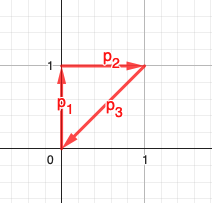
\includegraphics[width=5cm]{\CWD/andar-trebado-img.png}
    \caption{Exemplo do bêbado voltando para casa após três movimentos: N, L e SO}
\end{figure}

% For input, use one of the following
%

\inputdesc{A entrada é composta por dois inteiros $K$ ($1 \leq K \leq 5000$) e $P$ primo ($10^8 \leq P \leq 10^9$).}
%
% For output, use one of the following
%

\outputdesc{A saída deve ser composta por um único número: o número de formas que o bêbado pode voltar para a origem depois de $K$ movimentos módulo $P$.}

%\sampleio will look for files named sample-n.in and sample-n.sol (where n is 1, 2, 3...)
%in the documents directory and include them as samples.

\sampleio
